\documentclass[conference]{IEEEtran}
\IEEEoverridecommandlockouts

\usepackage{cite}
\usepackage{amsmath,amssymb,amsfonts}
\usepackage{graphicx}
\usepackage{booktabs}
\usepackage{multirow}
\usepackage{textcomp}
\usepackage{xcolor}
\usepackage{url}
\usepackage[hidelinks]{hyperref}
\graphicspath{{figures/}{../figures/}}
\hypersetup{pdftitle={Classifying Abalone Age Groups from Physical Measurements with Dense Neural Networks}}

\newcommand{\pmci}[2]{$#1 \pm #2$}

% Allow more and larger floats per page so figures stay near their text
\renewcommand{\topfraction}{0.9}
\renewcommand{\bottomfraction}{0.8}
\renewcommand{\textfraction}{0.07}
\renewcommand{\floatpagefraction}{0.85}
\renewcommand{\dbltopfraction}{0.8}
\renewcommand{\dblfloatpagefraction}{0.85}
\setcounter{topnumber}{3}
\setcounter{bottomnumber}{2}
\setcounter{totalnumber}{5}
\setcounter{dbltopnumber}{2}

\begin{document}

\title{Classifying Abalone Age Groups from Physical Measurements with Dense Neural Networks}

\author{}

\maketitle

\begin{abstract}
The age of an abalone is normally found by sectioning the shell, staining it and counting growth rings under a microscope. This report treats age estimation from cheaper physical measurements as a four-class classification problem (age $\le 7$, $7$--$10$, $10$--$15$ and $>15$ years) and solves it with dense neural networks trained in scikit-learn. After cleaning the UCI Abalone data and making a fixed, stratified 60/40 train/test split, I varied the number of hidden neurons, the learning rate, the number of hidden layers and the optimiser, repeating every configuration ten times from different initial weights. A network with one hidden layer of 20 ReLU neurons, trained with plain stochastic gradient descent (SGD) at a learning rate of 0.01 for 300 epochs, gave the best test accuracy of $72.10\% \pm 0.20\%$ (mean and 95\% confidence interval), against a majority-class baseline of 54.6\%. A second hidden layer did not change test accuracy ($p = 0.81$). Adam lowered the training loss faster but generalised slightly worse. The one-vs-rest areas under the ROC curve were 0.979, 0.881, 0.827 and 0.875 for the four classes. Most errors fall between neighbouring age groups, and the oldest group is the hardest to recognise because its measurements overlap heavily with those of the 10--15 year group.
\end{abstract}

\begin{IEEEkeywords}
neural networks, multilayer perceptron, stochastic gradient descent, Adam, classification, abalone
\end{IEEEkeywords}

\section{Introduction}

Abalone are marine snails of the genus \emph{Haliotis}, and studies of their populations need the age of each animal \cite{nash1994}. Age is found by cutting the shell through the cone, staining it and counting the rings under a microscope, which is slow and tedious \cite{uci}. The UCI Machine Learning Repository holds 4177 blacklip abalone from the Tasmanian survey of Nash \emph{et al.} \cite{nash1994}, with the sex, shell dimensions, several weights and ring count of each; records with missing values were removed before the data were donated \cite{uci}. If the easier measurements predict age well enough, they could replace the ring count for routine sorting.

Earlier machine-learning work on these data found the problem hard. Waugh \cite{waugh1995} reported test accuracies of 59--66\% for Cascade-Correlation networks, C4.5 and $k$-nearest neighbours on a three-class version of the task. The documentation that accompanies the data notes that the classes overlap heavily and that environmental information such as weather and food supply may be needed to separate them \cite{uci}. Those results suggest that accuracies well short of 100\% should be expected from these measurements whichever model is used.

Dense feedforward networks, also called multilayer perceptrons, are a natural choice for this kind of tabular problem. With enough hidden units a network with a single hidden layer can approximate any continuous function on a compact set \cite{cybenko1989,hornik1989}, and backpropagation gives an efficient way to compute the gradients needed to train it \cite{rumelhart1986}. In practice the result depends on a handful of design choices: the width and depth of the network, the learning rate, the optimiser and the length of training \cite{bengio2012,goodfellow2016}. Stochastic gradient descent is the classic optimiser for large-scale learning \cite{bottou2010}. Adam adapts a separate step size for every weight and usually converges faster \cite{kingma2015}, although adaptive methods can generalise worse than SGD on some problems \cite{wilson2017}.

The aim of this study is to build a dense neural network that assigns an abalone to one of four ring-age classes from its physical measurements, and to show how each design choice affects performance. The specific goals were to:
\begin{enumerate}
\item explore the data, including the class distribution and the distribution of every feature;
\item find the best number of hidden neurons (5, 10, 15 or 20) for a one-hidden-layer network trained with SGD;
\item measure the effect of the SGD learning rate;
\item test whether a second hidden layer helps;
\item compare Adam with SGD on training and test performance;
\item evaluate the final model with a confusion matrix, per-class ROC curves and the test accuracy.
\end{enumerate}

Section~\ref{sec:method} describes the data preparation, the network and the experimental design. Section~\ref{sec:results} reports and discusses the results, and Section~\ref{sec:conclusion} concludes.

\section{Methodology}\label{sec:method}

\subsection{Data and Cleaning}

The UCI file holds 4177 records with eight inputs: sex (male, female or infant), length, diameter, height and four weights (whole, shucked meat, viscera and dried shell). The continuous values were divided by 200 by the donors for use with neural networks \cite{uci}, so they are dimensionless in what follows. The target is the number of rings, and age in years is the ring count plus 1.5.

The file had no missing values and no duplicate rows. Two specimens had a height of zero, which is physically impossible. Two others had heights of 0.515 and 1.13 when the 99th percentile is about 0.22 and the next largest value is 0.25. Both lie far beyond Tukey's outer fence, $Q_3 + 3\,\mathrm{IQR}$ \cite{tukey1977}, and the 1.13 specimen would be taller than it is long, so all four were treated as recording errors and removed, leaving 4173 records. In 154 records the whole weight is slightly smaller than the sum of the shucked, viscera and shell weights. This is plausible because water is lost during shucking and drying, so these records were kept.

\subsection{Converting Age into Classes}

Age $a$ = rings $+\,1.5$ was mapped to four classes as set out in the task: class 1 for $a \le 7$, class 2 for $7 < a \le 10$, class 3 for $10 < a \le 15$ and class 4 for $a > 15$. Because ring counts are integers, this is the same as grouping 1--5, 6--8, 9--13 and 14 or more rings. The network therefore has four output neurons, one per class.

\begin{figure*}[t]
\centering
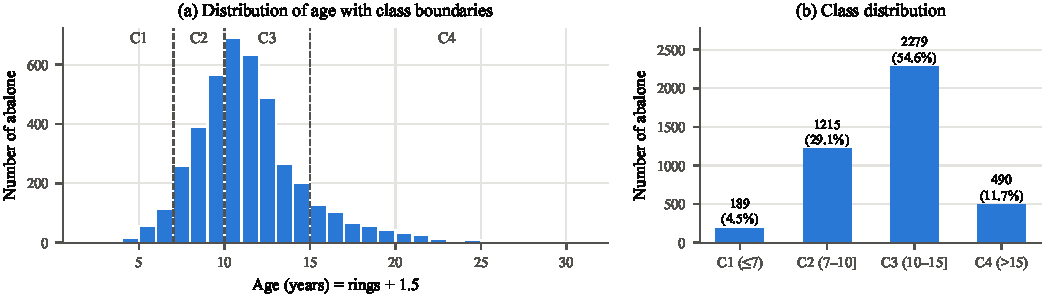
\includegraphics[width=\textwidth]{fig_class_distribution}
\caption{(a) Age (rings $+\,1.5$) after cleaning, with the class boundaries at 7, 10 and 15 years marked by dashed lines. (b) Number and share of abalone in each class ($N = 4173$).}
\label{fig:classes}
\end{figure*}

\subsection{Feature Preparation and Data Split}

Sex is nominal, so it was one-hot encoded into three binary inputs, which avoids imposing an artificial order on male, female and infant. Together with the seven continuous measurements this gives ten inputs. The data were split once into 60\% training (2503 records) and 40\% test (1670 records) with a fixed random seed. The split was stratified on the class label so that the rare class 1 (4.5\% of the data) appears in the same proportion in both parts. The same split was used for every experiment, so differences between configurations come only from the model and its initial weights.

The continuous inputs were standardised to zero mean and unit variance. Inputs on similar scales keep the error surface better conditioned and let a single learning rate suit all weights \cite{lecun1998}. The means and standard deviations were estimated on the training set only and then applied to the test set, so no information from the test data reached the model during training.

\subsection{Network Architecture}

The networks are fully connected feedforward networks built with the multilayer perceptron classifier (MLPClassifier) of scikit-learn 1.7.1 \cite{pedregosa2011}. Each hidden neuron uses the rectified linear unit (ReLU) \cite{nair2010}, $\mathrm{ReLU}(z) = \max(0, z)$, which avoids the vanishing gradients of saturating activations and is the scikit-learn default. The output layer has four neurons with the softmax function
\begin{equation}
\hat{p}_k = \frac{\exp(z_k)}{\sum_{j=1}^{4}\exp(z_j)}, \qquad k = 1,\dots,4,
\end{equation}
so the outputs are class probabilities and the predicted class is the one with the largest $\hat{p}_k$. The network is trained to minimise the cross-entropy loss over the $N$ training examples,
\begin{equation}
L(\mathbf{w}) = -\frac{1}{N}\sum_{i=1}^{N}\sum_{k=1}^{4} y_{ik}\log \hat{p}_{ik},
\end{equation}
where $y_{ik}$ is 1 if example $i$ belongs to class $k$ and 0 otherwise. Weights are initialised with the scaled uniform scheme of Glorot and Bengio \cite{glorot2010}. The random seed of each run fixes both the initial weights and the order of the mini-batches.

\begin{figure*}[t]
\centering
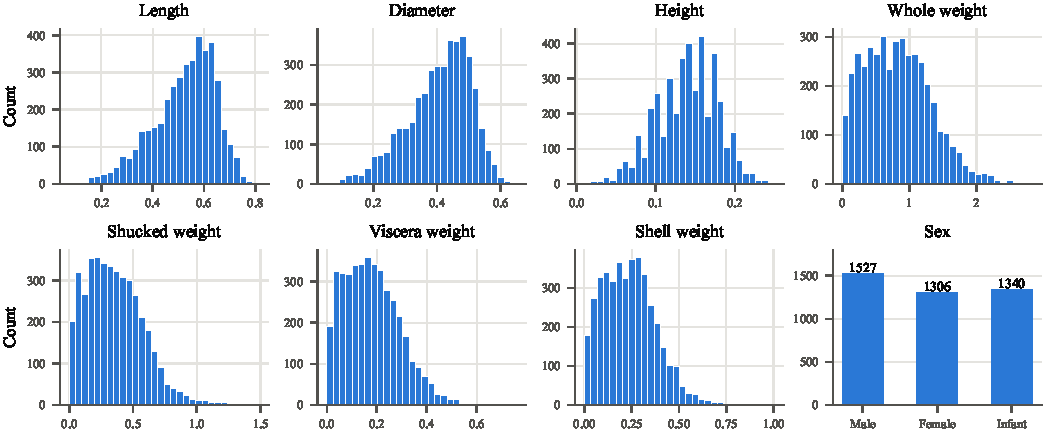
\includegraphics[width=\textwidth]{fig_feature_distributions}
\caption{Distribution of the seven continuous features (values as supplied, i.e., original units divided by 200) and counts of each sex, after cleaning.}
\label{fig:features}
\end{figure*}

\subsection{Optimisers}

SGD updates the weights after each mini-batch $B$ by
\begin{equation}
\mathbf{w} \leftarrow \mathbf{w} - \eta\, \nabla_{\mathbf{w}} L_B(\mathbf{w}),
\end{equation}
where $\eta$ is the learning rate and $L_B$ is the loss on the batch \cite{bottou2010}. I used plain SGD with a constant learning rate, with momentum and the L2 penalty both switched off. Nesterov momentum is on by default in scikit-learn, and turning it off means that Step~3 measures the learning rate on its own rather than the combined effect of the learning rate and momentum. Adam keeps running averages of the gradient and of its square and scales each weight's step by them \cite{kingma2015}. Its default learning rate, $\eta = 0.001$, was used, and Adam was also run at the best SGD learning rate for a like-for-like check. All models used mini-batches of 32 examples, which gives about 78 weight updates per epoch on the training set.

\subsection{Choosing the Training Length}

There was no validation set, so the number of epochs was fixed in advance from a convergence trial rather than tuned by early stopping. A network with ten hidden neurons was trained for 1000 epochs, three times each with SGD at $\eta = 0.01$, SGD at $\eta = 0.1$ and Adam at $\eta = 0.001$, while recording the train and test loss after every epoch. The results are discussed in Section~\ref{sec:conv}. On that basis every later experiment used a budget of 300 epochs.

\begin{figure*}[t]
\centering
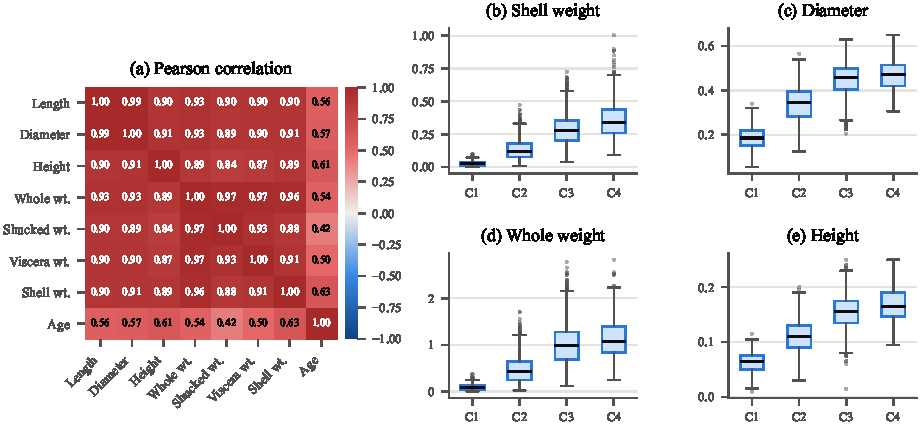
\includegraphics[width=\textwidth]{fig_corr_boxes}
\caption{(a) Pearson correlation between the continuous features and age. (b)--(e) Four of the most age-related features by class (original units divided by 200). The spread within each class is large, and classes 3 and 4 overlap almost completely.}
\label{fig:corrbox}
\end{figure*}

\subsection{Experimental Design and Evaluation}

The experiments followed the steps of the task, and each step used the best setting found in the step before. Step~2 compared one hidden layer of 5, 10, 15 and 20 neurons with SGD at $\eta = 0.01$, a common starting value \cite{bengio2012}. Step~3 varied $\eta$ over $\{0.001, 0.005, 0.01, 0.05, 0.1, 0.2\}$ with the best width. Step~4 added a second hidden layer of the same width with the best $\eta$. Step~5 compared SGD with Adam on the best architecture, and Step~6 evaluated the final model in detail.

Every configuration was trained ten times with seeds 0 to 9. For each metric I report the mean over the ten runs and the half-width of a 95\% confidence interval from the $t$ distribution,
\begin{equation}
\bar{x} \pm t_{0.975,\,9}\,\frac{s}{\sqrt{10}}, \qquad t_{0.975,\,9} = 2.262,
\end{equation}
where $s$ is the sample standard deviation. Where two configurations were close, I compared their ten test accuracies with Welch's $t$-test.

Accuracy on the train and test sets is the main metric because the task asks for it. The classes are imbalanced, however, and a model that always predicted class 3 would already score 54.6\% on the test set \cite{he2009}. I therefore also report the macro-averaged F1 score, which weights the four classes equally. The final model is described with a confusion matrix, per-class precision, recall and F1, and one-vs-rest ROC curves with their areas under the curve (AUC) \cite{fawcett2006,hand2001}. A configuration was taken to be better if its mean test accuracy was higher. When two configurations were statistically indistinguishable, I kept the simpler one.

\begin{figure*}[t]
\centering
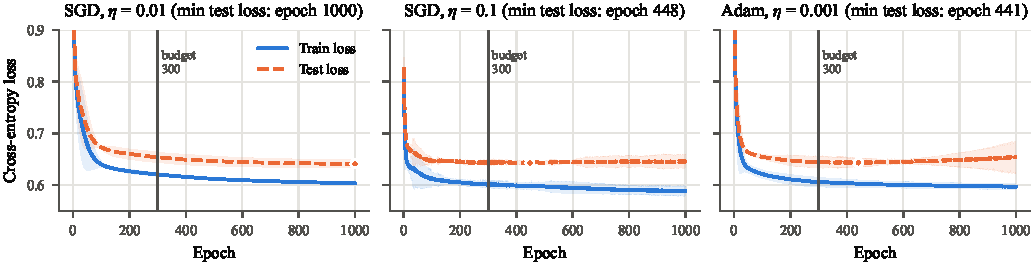
\includegraphics[width=\textwidth]{fig_convergence}
\caption{Convergence trial: train and test cross-entropy loss over 1000 epochs for a network with ten hidden neurons (mean of three runs, shaded band shows the 95\% CI). The vertical line marks the 300-epoch budget and the dot marks the lowest mean test loss.}
\label{fig:convergence}
\end{figure*}

\section{Results and Discussion}\label{sec:results}

\subsection{Data Exploration}

Fig.~\ref{fig:classes} shows the age distribution and the four classes. Age is right-skewed (skewness 1.11), with a mode near 10.5 years and a long tail up to 30.5 years. Class 3 holds more than half of the abalone (54.6\%), class 2 holds 29.1\%, class 4 holds 11.7\% and class 1 only 4.5\%. With 189 examples in class 1 and 490 in class 4, the two outer classes are the ones most at risk of being under-predicted.

The feature distributions are shown in Fig.~\ref{fig:features}. Length and diameter are left-skewed (skewness $-0.64$ and $-0.61$), while the four weights are right-skewed (0.53 to 0.72). Once the outliers were removed, height is close to symmetric. The three sexes are roughly balanced (1527 male, 1306 female and 1340 infant). Sex is informative about age. Of the infants, 68.6\% fall in classes 1 and 2, while 85.9\% of females and 80.4\% of males fall in classes 3 and 4.

Fig.~\ref{fig:corrbox}(a) shows that the physical measurements are strongly correlated with one another ($r = 0.84$ to $0.99$), so they carry much the same information about the overall size of the animal. Their correlations with age are only moderate, from 0.42 for shucked weight to 0.63 for shell weight. The box plots in Fig.~\ref{fig:corrbox}(b)--(e) show why. Each feature rises with age group, but the boxes of classes 3 and 4 overlap almost completely. Once an abalone stops growing quickly, its size says little about how many more years it has lived, so no model built on these inputs is likely to separate the older classes cleanly.

\begin{table*}[t]
\centering
\caption{Mean and 95\% confidence interval over ten runs for every configuration (300 epochs, batch size 32). The selected setting in each step is in bold.}
\label{tab:results}
\footnotesize
\setlength{\tabcolsep}{5pt}
\begin{tabular}{llcccc}
\toprule
Step & Configuration & Parameters & Train accuracy (\%) & Test accuracy (\%) & Test macro-F1 \\
\midrule
\multirow{4}{*}{2. Hidden neurons} & 1 layer, 5 neurons, SGD $\eta=0.01$ & 79 & \pmci{73.23}{0.15} & \pmci{71.44}{0.40} & \pmci{0.631}{0.005} \\
 & 1 layer, 10 neurons, SGD $\eta=0.01$ & 154 & \pmci{73.36}{0.22} & \pmci{71.86}{0.40} & \pmci{0.633}{0.004} \\
 & 1 layer, 15 neurons, SGD $\eta=0.01$ & 229 & \pmci{73.53}{0.22} & \pmci{71.97}{0.22} & \pmci{0.636}{0.004} \\
 & \textbf{1 layer, 20 neurons, SGD $\boldsymbol{\eta=0.01}$} & 304 & \pmci{73.58}{0.12} & \pmci{\mathbf{72.10}}{0.20} & \pmci{0.638}{0.004} \\
\midrule
\multirow{6}{*}{3. Learning rate} & 1 layer, 20 neurons, SGD $\eta=0.001$ & 304 & \pmci{71.53}{0.37} & \pmci{69.95}{0.59} & \pmci{0.575}{0.018} \\
 & 1 layer, 20 neurons, SGD $\eta=0.005$ & 304 & \pmci{73.36}{0.19} & \pmci{71.67}{0.19} & \pmci{0.629}{0.002} \\
 & \textbf{1 layer, 20 neurons, SGD $\boldsymbol{\eta=0.01}$} & 304 & \pmci{73.58}{0.12} & \pmci{\mathbf{72.10}}{0.20} & \pmci{0.638}{0.004} \\
 & 1 layer, 20 neurons, SGD $\eta=0.05$ & 304 & \pmci{73.62}{0.33} & \pmci{71.97}{0.41} & \pmci{0.644}{0.006} \\
 & 1 layer, 20 neurons, SGD $\eta=0.1$ & 304 & \pmci{73.48}{0.41} & \pmci{71.28}{0.69} & \pmci{0.639}{0.006} \\
 & 1 layer, 20 neurons, SGD $\eta=0.2$ & 304 & \pmci{73.51}{0.67} & \pmci{70.68}{0.85} & \pmci{0.636}{0.010} \\
\midrule
4. Hidden layers & 2 layers, 20 + 20 neurons, SGD $\eta=0.01$ & 724 & \pmci{73.80}{0.21} & \pmci{72.06}{0.34} & \pmci{0.644}{0.006} \\
\midrule
\multirow{2}{*}{5. Optimiser} & 1 layer, 20 neurons, Adam $\eta=0.001$ & 304 & \pmci{74.02}{0.17} & \pmci{71.84}{0.20} & \pmci{0.639}{0.003} \\
 & 1 layer, 20 neurons, Adam $\eta=0.01$ & 304 & \pmci{74.75}{0.33} & \pmci{71.28}{0.52} & \pmci{0.643}{0.010} \\
\bottomrule
\end{tabular}
\end{table*}

\begin{figure*}[t]
\centering
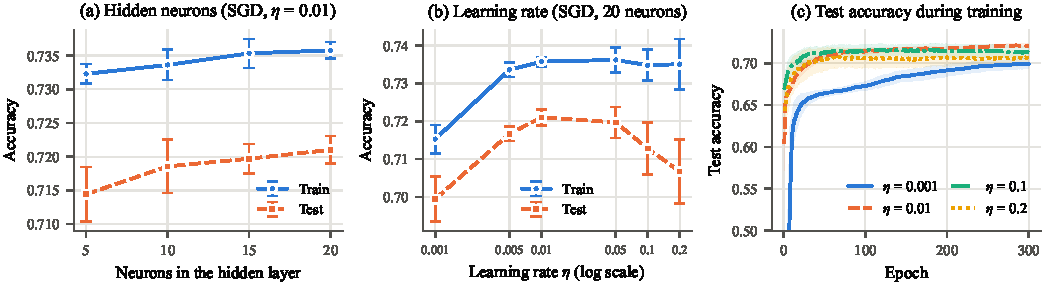
\includegraphics[width=\textwidth]{fig_step2_step3}
\caption{Train and test accuracy (mean and 95\% CI over ten runs) for (a) the number of hidden neurons and (b) the SGD learning rate with 20 hidden neurons. (c) Test accuracy during training for four of those learning rates (mean of ten runs with 95\% CI bands).}
\label{fig:steps23}
\end{figure*}

\subsection{Convergence Trial and Training Budget}\label{sec:conv}

Fig.~\ref{fig:convergence} shows the convergence trial. With SGD at $\eta = 0.01$ the test loss falls quickly for about 100 epochs and then keeps falling slowly up to epoch 1000. Test accuracy was 71.5\% at epoch 300 and 72.2\% at epoch 1000. With SGD at $\eta = 0.1$ and with Adam the test loss reaches its minimum near epochs 448 and 441 respectively and then creeps upwards while the training loss keeps falling, which is the usual sign of overfitting. At epoch 300 their test losses are within 0.002 of those minima. A budget of 300 epochs therefore lets the faster settings converge without letting them overfit, and leaves the slower settings within about 0.6 percentage points of their final accuracy. Training for longer would mainly favour small learning rates and would cost more than three times as much computation.

\begin{figure*}[t]
\centering
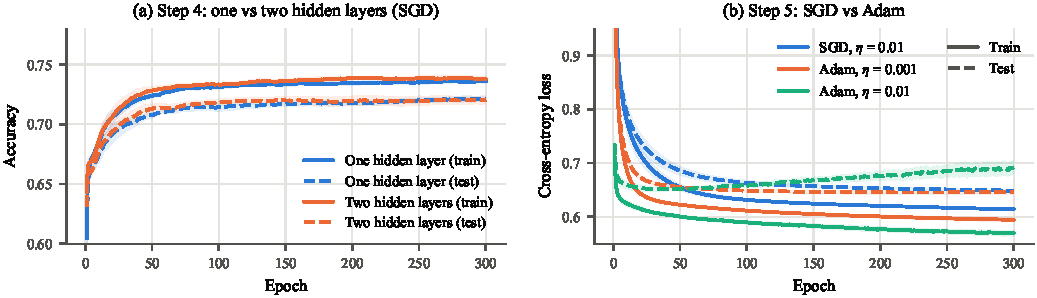
\includegraphics[width=\textwidth]{fig_step4_step5}
\caption{(a) Train (solid) and test (dashed) accuracy with one and two hidden layers of 20 neurons, SGD $\eta = 0.01$. (b) Train and test cross-entropy loss for SGD and Adam with one hidden layer of 20 neurons. Curves show the mean of ten runs with 95\% CI bands.}
\label{fig:steps45}
\end{figure*}

\subsection{Step 2: Number of Hidden Neurons}

Table~\ref{tab:results} and Fig.~\ref{fig:steps23}(a) give the results for one hidden layer trained with SGD at $\eta = 0.01$. Test accuracy rises steadily with width, from 71.44\% with five neurons to 72.10\% with twenty, and macro-F1 follows the same pattern. Twenty neurons is clearly better than five (Welch's $t$-test, $p = 0.006$), but the gains flatten out: the difference between 15 and 20 neurons is within the run-to-run noise ($p = 0.33$). The gap between train and test accuracy stays near 1.5 percentage points at every width, so even the largest network, with 304 weights for 2503 training examples, shows no sign of overfitting within 300 epochs. A five-neuron network appears slightly too small to capture the non-linear relationship between size and age, while beyond 15 neurons extra capacity brings little. Twenty neurons was selected as the best of the values considered.

\subsection{Step 3: Learning Rate}

The learning rate had a larger effect than the width (Fig.~\ref{fig:steps23}(b)). At $\eta = 0.001$ the network is still learning when training stops (Fig.~\ref{fig:steps23}(c)). It reaches only 69.95\% test accuracy and the lowest macro-F1 of any model (0.575), because it has not yet learned to predict the small classes. Accuracy peaks at $\eta = 0.01$ (72.10\%), with $\eta = 0.05$ statistically tied (71.97\%, $p = 0.53$). Above that, test accuracy falls to 71.28\% at $\eta = 0.1$ and 70.68\% at $\eta = 0.2$ while training accuracy barely changes. The confidence intervals also widen about fourfold, from $\pm 0.20$ to $\pm 0.85$ points. Large steps make each run end at a different point of a noisy trajectory, so the final model depends more on the seed and generalises less consistently. In the convergence trial a larger rate also reached its best test loss sooner and then began to overfit. Since $\eta = 0.01$ gave the highest mean test accuracy and the narrowest interval, it was kept for the remaining steps. The slightly higher macro-F1 at $\eta = 0.05$ (0.644 against 0.638) suggests that larger rates help a little with the minority classes, but the difference is within one confidence interval.

\begin{figure*}[t]
\centering
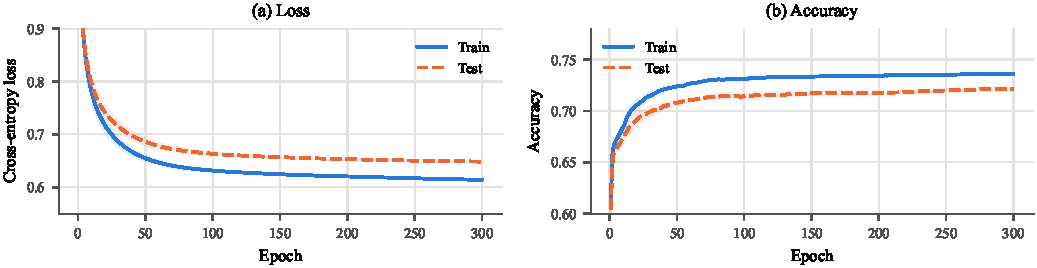
\includegraphics[width=\textwidth]{fig_final_curves}
\caption{Learning curves of the final model (one hidden layer of 20 neurons, SGD $\eta = 0.01$): (a) cross-entropy loss and (b) accuracy on the train and test sets (mean of ten runs with 95\% CI bands).}
\label{fig:final}
\end{figure*}

\subsection{Step 4: Number of Hidden Layers}

Adding a second hidden layer of 20 neurons raised training accuracy from 73.58\% to 73.80\% but left test accuracy unchanged (72.06\% against 72.10\%, $p = 0.81$). The learning curves of the two networks are almost on top of each other (Fig.~\ref{fig:steps45}(a)). The deeper network has more than twice as many weights (724 against 304) and a slightly wider generalisation gap (1.74 against 1.48 points). With ten inputs that are themselves highly correlated, one hidden layer appears to have enough capacity, and universal approximation results show that a single hidden layer is sufficient in principle \cite{cybenko1989,hornik1989}. The test macro-F1 of the deeper network was slightly higher (0.644 against 0.638), but again by less than its confidence interval. Following the rule of keeping the simpler of two equivalent models, the one-hidden-layer network was carried forward.

\begin{figure*}[t]
\centering
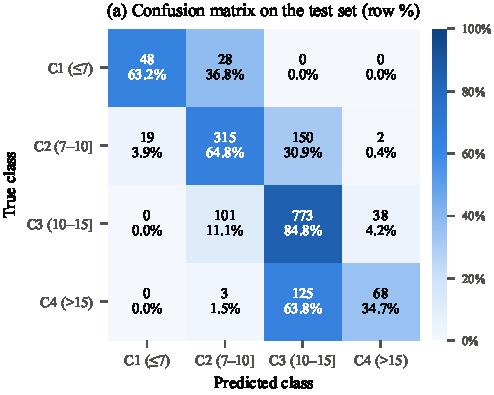
\includegraphics[width=0.49\textwidth]{fig_confusion_matrix}\hfill
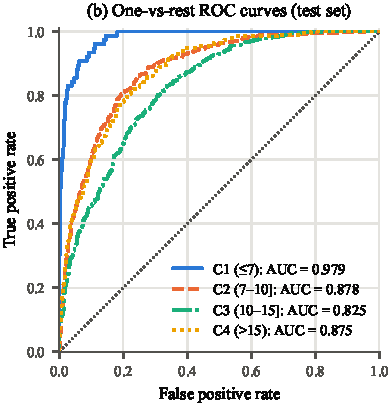
\includegraphics[width=0.43\textwidth]{fig_roc}
\caption{Final model on the test set. (a) Confusion matrix; each cell gives the count and the percentage of its true class (row). (b) One-vs-rest ROC curves; AUCs in the legend are for this run and the dotted diagonal is a random classifier. Both panels are for the representative run.}
\label{fig:cmroc}
\end{figure*}

\subsection{Step 5: Adam versus SGD}

Fig.~\ref{fig:steps45}(b) shows the main difference between the optimisers. Adam lowers the training loss much faster than SGD and ends with a lower training loss, giving the highest training accuracies in the study (74.02\% at $\eta = 0.001$ and 74.75\% at $\eta = 0.01$). That advantage does not carry over to the test set. Adam at $\eta = 0.001$ is within 0.004 of its lowest test loss by epoch 100 and changes little after that, finishing at 71.84\% test accuracy, a little below SGD ($p = 0.055$). At $\eta = 0.01$ Adam's test loss starts rising after roughly 30 epochs while its training loss keeps falling, and its test accuracy drops to 71.28\% ($p = 0.006$ against SGD). Its generalisation gap of 3.5 points is more than twice that of SGD (1.5 points). This matches the observation of Wilson \emph{et al.} \cite{wilson2017} that adaptive methods can fit the training data faster but find solutions that generalise worse than plain SGD. With a fixed budget and no regularisation, SGD at $\eta = 0.01$ was the better optimiser here. Adam would be the more efficient choice if training were stopped early, for example after 50 to 100 epochs, since by then it is already close to its best test loss.

\subsection{Step 6: Final Model}

The final model is a network with ten inputs, one hidden layer of 20 ReLU neurons and four softmax outputs, trained with plain SGD ($\eta = 0.01$, batch size 32) for 300 epochs. Over ten runs its test accuracy was $72.10\% \pm 0.20\%$ (range 71.56\% to 72.46\%) and its train accuracy $73.58\% \pm 0.12\%$. Fig.~\ref{fig:final} shows its learning curves. The train and test curves stay close together throughout, so the model does not overfit. The detailed results below are for the run whose test accuracy was closest to the ten-run mean (seed 5, 72.10\% test accuracy).

The confusion matrix (Fig.~\ref{fig:cmroc}(a)) shows that almost every error is between neighbouring age groups. Only five of the 1670 test abalone were assigned to a class two steps away, and none three steps away. Class 3 is recognised best (recall 84.8\%), helped by being the largest class. Class 4 is the weakest. Only 34.7\% of the oldest abalone are identified, and 63.8\% are labelled as class 3, which agrees with the overlap seen in Fig.~\ref{fig:corrbox}. Class 1 is small but well defined, and its errors all go to class 2. Table~\ref{tab:perclass} lists the per-class metrics.

\begin{table}[!t]
\centering
\caption{Per-class test metrics of the final model. Precision, recall and F1 are from the representative run; AUC is the mean and 95\% CI over ten runs.}
\label{tab:perclass}
\footnotesize
\setlength{\tabcolsep}{3.5pt}
\begin{tabular}{lccccc}
\toprule
Class & $n$ & Precision & Recall & F1 & AUC \\
\midrule
1 (age $\le 7$) & 76 & 0.716 & 0.632 & 0.671 & \pmci{0.979}{0.001} \\
2 ($7 < a \le 10$) & 486 & 0.705 & 0.648 & 0.675 & \pmci{0.881}{0.001} \\
3 ($10 < a \le 15$) & 912 & 0.738 & 0.848 & 0.789 & \pmci{0.827}{0.002} \\
4 (age $> 15$) & 196 & 0.630 & 0.347 & 0.447 & \pmci{0.875}{0.002} \\
\midrule
Macro average & 1670 & 0.697 & 0.619 & 0.646 & 0.891 \\
\bottomrule
\end{tabular}
\end{table}

The one-vs-rest ROC curves (Fig.~\ref{fig:cmroc}(b)) show that the network ranks examples well even where its hard predictions are weak. Averaged over the ten runs, class 1 is almost perfectly separable (AUC 0.979). Classes 2 and 4 have AUCs of 0.881 and 0.875, and class 3 has the lowest AUC (0.827) because it sits in the middle of the age range and is confused with both neighbours. The AUC of 0.875 for class 4, against a recall of only 34.7\%, means that the oldest abalone do receive higher class-4 probabilities than the rest, but those probabilities rarely exceed the class-3 probability. Lowering the decision threshold for class 4, or reweighting the classes during training \cite{he2009}, should raise its recall at some cost in precision. The AUCs varied very little between runs (CI half-widths of 0.002 or less), so the ranking ability is stable across initialisations.

\subsection{Limitations}

As the task specified, there was no validation set, so the hyperparameters were chosen on the same test set used to report performance. The reported 72.10\% is therefore slightly optimistic, although the leading configurations differed so little that the bias is probably a fraction of a percentage point. The class labels are ordered, but cross-entropy treats them as unrelated categories, and an ordinal loss could make better use of that structure. The class imbalance was left untreated so that accuracy would reflect the natural class frequencies, which is why class 4 recall is low. Lastly, the fixed 300-epoch budget slightly favours learning rates that converge quickly, which is part of the reason $\eta = 0.001$ performed poorly.

\section{Conclusion}\label{sec:conclusion}

This study built dense neural networks that classify abalone into four ring-age groups from sex and seven physical measurements. A single hidden layer of 20 ReLU neurons trained with plain SGD at $\eta = 0.01$ for 300 epochs gave the best test accuracy, $72.10\% \pm 0.20\%$ over ten runs, compared with 54.6\% for always predicting the largest class. Width mattered up to about 15 neurons. The learning rate mattered more: too small a rate left the network undertrained within the budget, and too large a rate made results noisier and less accurate. A second hidden layer added parameters without improving test performance. Adam fitted the training data faster, but with no regularisation it generalised slightly worse than SGD and overfitted at the larger learning rate.

The final model makes almost all of its errors between neighbouring age groups and separates the youngest abalone very well (AUC 0.979). Its main weakness is the oldest group, whose size and weight overlap with those of the 10--15 year group, so only about a third of these abalone are recognised. The exploratory analysis suggests that this limit comes from the measurements rather than from the network. Further gains are more likely to come from information the data lack, such as location or environmental conditions, as the data documentation suggests \cite{uci}, and from methods that address imbalance and class order, than from larger networks. Future work could tune hyperparameters with a separate validation set and early stopping, apply class weighting or threshold adjustment for the minority classes, and compare an ordinal loss with standard cross-entropy.

\begin{thebibliography}{99}

\bibitem{nash1994}
W. J. Nash, T. L. Sellers, S. R. Talbot, A. J. Cawthorn, and W. B. Ford, ``The population biology of abalone (\emph{Haliotis} species) in Tasmania. I. Blacklip abalone (\emph{H. rubra}) from the north coast and islands of Bass Strait,'' Sea Fisheries Division, Tasmania, Tech. Rep. 48, 1994.

\bibitem{uci}
W. Nash, T. Sellers, S. Talbot, A. Cawthorn, and W. Ford, ``Abalone,'' UCI Machine Learning Repository, 1994. [Online]. Available: https://doi.org/10.24432/C55C7W

\bibitem{waugh1995}
S. G. Waugh, ``Extending and benchmarking Cascade-Correlation: Extensions to the Cascade-Correlation architecture and benchmarking of feed-forward supervised artificial neural networks,'' Ph.D. dissertation, Dept. Comput. Sci., Univ. Tasmania, Hobart, Australia, 1995.

\bibitem{cybenko1989}
G. Cybenko, ``Approximation by superpositions of a sigmoidal function,'' \emph{Math. Control, Signals, Syst.}, vol. 2, no. 4, pp. 303--314, 1989.

\bibitem{hornik1989}
K. Hornik, M. Stinchcombe, and H. White, ``Multilayer feedforward networks are universal approximators,'' \emph{Neural Netw.}, vol. 2, no. 5, pp. 359--366, 1989.

\bibitem{rumelhart1986}
D. E. Rumelhart, G. E. Hinton, and R. J. Williams, ``Learning representations by back-propagating errors,'' \emph{Nature}, vol. 323, no. 6088, pp. 533--536, 1986.

\bibitem{bengio2012}
Y. Bengio, ``Practical recommendations for gradient-based training of deep architectures,'' in \emph{Neural Networks: Tricks of the Trade}, 2nd ed., G. Montavon, G. B. Orr, and K.-R. M\"{u}ller, Eds. Berlin, Germany: Springer, 2012, pp. 437--478.

\bibitem{goodfellow2016}
I. Goodfellow, Y. Bengio, and A. Courville, \emph{Deep Learning}. Cambridge, MA, USA: MIT Press, 2016.

\bibitem{bottou2010}
L. Bottou, ``Large-scale machine learning with stochastic gradient descent,'' in \emph{Proc. COMPSTAT'2010}, Paris, France, 2010, pp. 177--186.

\bibitem{kingma2015}
D. P. Kingma and J. Ba, ``Adam: A method for stochastic optimization,'' in \emph{Proc. 3rd Int. Conf. Learn. Represent. (ICLR)}, San Diego, CA, USA, 2015.

\bibitem{wilson2017}
A. C. Wilson, R. Roelofs, M. Stern, N. Srebro, and B. Recht, ``The marginal value of adaptive gradient methods in machine learning,'' in \emph{Advances in Neural Information Processing Systems 30}, 2017, pp. 4148--4158.

\bibitem{tukey1977}
J. W. Tukey, \emph{Exploratory Data Analysis}. Reading, MA, USA: Addison-Wesley, 1977.

\bibitem{lecun1998}
Y. LeCun, L. Bottou, G. B. Orr, and K.-R. M\"{u}ller, ``Efficient BackProp,'' in \emph{Neural Networks: Tricks of the Trade}, G. B. Orr and K.-R. M\"{u}ller, Eds. Berlin, Germany: Springer, 1998, pp. 9--50.

\bibitem{pedregosa2011}
F. Pedregosa \emph{et al.}, ``Scikit-learn: Machine learning in Python,'' \emph{J. Mach. Learn. Res.}, vol. 12, pp. 2825--2830, 2011.

\bibitem{nair2010}
V. Nair and G. E. Hinton, ``Rectified linear units improve restricted Boltzmann machines,'' in \emph{Proc. 27th Int. Conf. Mach. Learn. (ICML)}, Haifa, Israel, 2010, pp. 807--814.

\bibitem{glorot2010}
X. Glorot and Y. Bengio, ``Understanding the difficulty of training deep feedforward neural networks,'' in \emph{Proc. 13th Int. Conf. Artif. Intell. Statist. (AISTATS)}, Sardinia, Italy, 2010, pp. 249--256.

\bibitem{he2009}
H. He and E. A. Garcia, ``Learning from imbalanced data,'' \emph{IEEE Trans. Knowl. Data Eng.}, vol. 21, no. 9, pp. 1263--1284, 2009.

\bibitem{fawcett2006}
T. Fawcett, ``An introduction to ROC analysis,'' \emph{Pattern Recognit. Lett.}, vol. 27, no. 8, pp. 861--874, 2006.

\bibitem{hand2001}
D. J. Hand and R. J. Till, ``A simple generalisation of the area under the ROC curve for multiple class classification problems,'' \emph{Mach. Learn.}, vol. 45, no. 2, pp. 171--186, 2001.

\end{thebibliography}


\end{document}
